\section{Étude de coûts}


\paragraph{Descriptif de la pièce}
La pièce que nous considérons est une pièce relativement simple.
Il s'agit d'un couvercle anti-ingénierie inverse pour lecteur de carte de crédit.
Le rôle de cette pièce est de détecter toute tentative d'accéder à l'intérieur de l'appareil, soit en le démontant, soit en le perçant.
Pour accomplir cette fonction, deux pistes sont placées en serpentin à l'intérieur du couvercle.
L'appareil est programmé pour effacer toute les données sensibles dès qu'une de ces pistes est rompue.
Cette pièce était malheureusement confidentielle et nous n'avons pas pu la prendre en photo.
Néanmoins une vue simplifiée est visible à la fig. \ref{fig:example-part}.

\begin{figure}[h]
    \begin{center}
%        \missingfigure[figwidth=\textwidth]{Image de la pièce d'exemple.}
        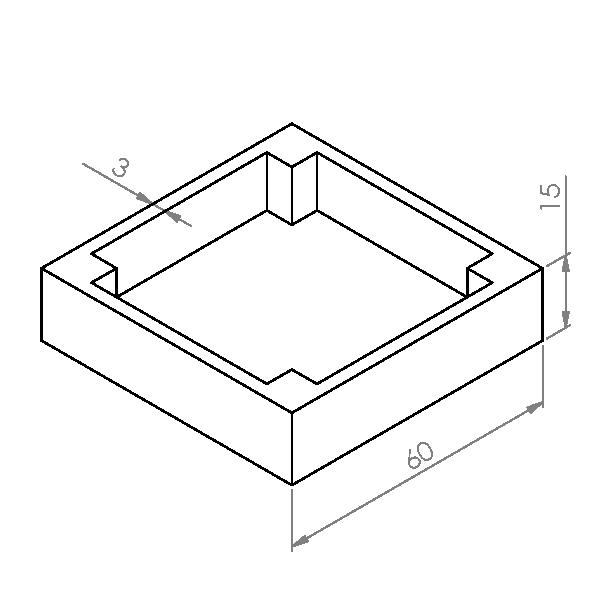
\includegraphics[width=\textwidth]{images/example_part/example_mid}
        \caption{Pièce d'exemple}\label{fig:example-part}
    \end{center}
\end{figure}
\subsection{Injection}
\begin{table}[h!]
\centering 
\begin{tabular}{l S[table-format=3.2] r} 
\toprule 
\multicolumn{2}{l}{\textbf{Électricité}} & \\ 
Consommation électrique & 5 & \si{\kilo\watt} \\
Prix de l'électricité & 0.2 & \si{\chf\per\kilo\watt\per\hour} \\
\cmidrule(l){2-3}
Coût d'électricité & 1 & \si{\chf\per\hour} \\
\midrule
\multicolumn{2}{l}{\textbf{Machines}} & \\ 
Presse électrique & 130000 & \si{\chf} \\
Fonctionnement & 6240 & \si{\hour\per\annee} \\
\cmidrule(l){2-3}
Amortissement sur 5 ans & 4.17 & \si{\chf\per\hour} \\
\midrule
\multicolumn{2}{l}{\textbf{Opérateurs}} & \\ 
Opérateur à 10\% & 6& \si{\chf\per\hour} \\
\midrule

\multicolumn{2}{l}{\textbf{Matière}} & \\ 
Matière (\textsc{pc}) & 11 & \si{\chf\per\kilogram} \\ 
Poids de la pièce & 25 & \si{\gram} \\
\cmidrule(l){2-3}
Coût de la matière & 0.27 & \si{\chf\per\piece} \\

\midrule
\multicolumn{2}{l}{\textbf{Outillage}} & \\ 
Prix du moule & 20000 & \si{\chf} \\
Pièces par série & 20000& \si{\piece} \\
\cmidrule(l){2-3}
Coûts d'outillage & 1 & \si{\chf\per\piece} \\

\midrule
\midrule
Coût horaire & 11.67  & \si{\chf\per\hour} \\
Temps de cycle & 20 & \si{\second\per\piece} \\
\cmidrule(l){2-3}
\textbf{\textsc{Total}} & 1.34 & \si{\chf\per\piece} \\

\bottomrule 
\end{tabular}
\caption{Calcul des coûts de l'injection plastique} 
\label{tab:cost-molding}
\end{table}




\subsection{Activation Laser}
Pour calculer le coût de l'étape d'activation sélective (\textsc{lds}) nous avons utilisés les hypothèses de départ suivantes :
\begin{itemize}
    \item Le secteur d'activation laser tourne \SI{24}{\hour} par jour, 5 jours sur 7.
    \item La machine est une Microline 160i de chez LPKF coûtant \SI{220000}{\chf}.
        Elle est amortie en 5 ans.
    \item Un opérateur ne peut s'occuper que d'une machine à la fois.
    \item Le temps de cycle est de \SI{25}{\second\per\piece}.
        Ce temps change très peu suivant la complexité des connexions électriques car la majorité du temps est prise utilisée pour la mise en place de la pièce et l'alignement visuel par la machine.
    \item La machine consomme en permanence sa puissance de pointe soit \SI{2.5}{\kilo\watt} \cite{lpkf-microline-series}.
        L'électricité représentant une fraction faible du coût final, cette hypothèse n'induis pas de grande erreurs.
\end{itemize}

Ces hypothèses sont basées sur ce que nous avons eu l'occasion de voir lors de notre visite chez Cicorel.
Elle s'appliquent à la production d'un couvercle anti-ingénierie inverse pour lecteur de carte.
Le seul facteur qui change pour une autre pièce est le temps d'illumination laser, qui représente une fraction du temps de cycle.
Les résultats du tab. \ref{tab:cost-laser-activation} sont donc valables pour la pluspart des pièces.

\begin{table}[h!]
\centering 
\begin{tabular}{l S[table-format=3.2] r} 
\toprule 
\multicolumn{2}{l}{\textbf{Électricité}} & \\ 
Consommation électrique & 2.5 & \si{\kilo\watt} \\
Prix de l'électricité & 0.2 & \si{\chf\per\kilo\watt\per\hour} \\
\cmidrule(l){2-3}
Prix de l'électricité & 0.5 & \si{\chf\per\hour} \\
\midrule
\multicolumn{2}{l}{\textbf{Machines}} & \\ 
LPKF Microline 160i & 220000 & \si{\chf} \\
Fonctionnement & 6240 & \si{\hour\per\annee} \\
\cmidrule(l){2-3}
Amortissement sur 5 ans& 7.05 & \si{\chf\per\hour} \\
\midrule
\multicolumn{2}{l}{\textbf{Opérateurs}} & \\ 
Opérateur à 100\% & 60& \si{\chf\per\hour} \\

\midrule
\multicolumn{2}{l}{\textbf{Temps de cycle}} & \\ 
Vitesse du laser & 4000 & \si{\milli\meter\per\second} \\
Diamètre du laser & 80 & \si{\micro\meter} \\
Vitesse de balayage & 320 & \si{\milli\meter\squared\per\second} \\
Surface des pistes & 1800 & \si{\milli\meter\squared\per\piece} \\ 
Temps de balayage & 5.625 & \si{\second\per\piece} \\ 
Temps de positionnement & 1 & \si{\second\per orientation} \\
Nombre d'orientations & 5 &  \\
Temps de mise en place, retrait et inspection & 15 & \si{\second\per\piece} \\ 

\cmidrule(l){2-3}
\textbf{Temps total} & 25.625 & \si{\second\per\piece} \\ 

\midrule
\midrule
Coût horaire & 67.68 & \si{\chf\per\hour} \\
Temps de cycle & 25.625 & \si{\second\per\piece} \\
\cmidrule(l){2-3}
\textbf{\textsc{Total}} & 0.48 & \si{\chf\per\piece} \\

\bottomrule 
\end{tabular}
\caption{Calcul des coûts de l'activation sélective par laser} 
\label{tab:cost-laser-activation}
\end{table}

